\section{Antenna Design 1 -- Minimized Monopole}
\label{sec:techsol1_monopole_5mm}
\begin{aautop}
As described in the chapter intro \ref{cha_intro_5mm}, this section will document the minimized monopole antenna. The documentation will contain a simulation both on the ground clearence test and the final minimized design.      
\end{aautop}

The minimized monopole design can be seen on Figure \fixme{3d figure}. The design is still based on the first folded monopole design, but is made smaller and simpler without any folding.

The ground clearence S11 and efficiency simulation can be seen on Figure \ref{fig:eff_s11_mono_sim_5mm}.
The simulation sweep is done from \SI{10}{mm} to \SI{3}{mm} ground clearence in \SI{1}{mm} steps and only for the top antenna. Each ground clearence simulation is matched and tuned to get the highest bandwidth possible.

From the S11 results it is clear that the bandwidth decreases as the ground clearence decreases. The most noticeable results is at \SI{5}{mm} clearence as the bandwidth from this point does not increase significantly when increasing the ground clearence. However decreasing the ground clearence further to \SI{4}{mm} and \SI{3}{mm} the bandwidth drops significantly. Based on these results is was chosen to minimize the antenna design to a ground clearence of \SI{5}{mm}.

The effieicncy ground clearence comparison shows some similar results. In the high band it's clear that decresing the ground clearence will also decrease the bandwidth. However the high band results seems hard to compare, as the different simulations is matched at different frequencies to gain the highest bandwidth. The comparison is more noticeable in the low band, where it is clear, that the lower the clearence the lower the efficiency. Generally the effieicncy does not drop that much when decreasing the ground clearence. It should also be possible to increase the efficiency and compensated for the drop with tuning.  

\begin{figure}[htbp]
   \begin{subfigure}[b]{0.49\linewidth}
        \centering
        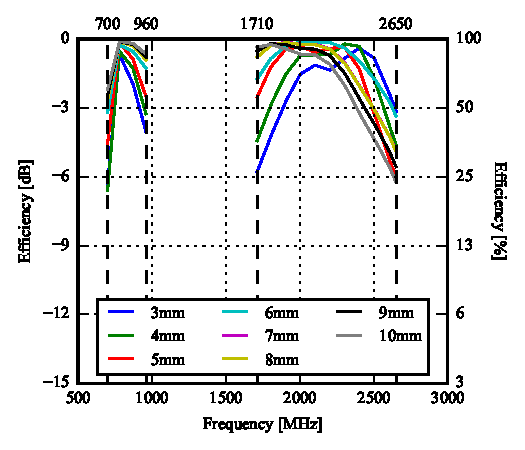
\includegraphics{img/tech_sol/monopole/5mm/eff_5mm}
        \caption{S11 parameter for the top antenna, when sweeping the ground clearence.}
        \label{fig:s11_mono_sim_5mm}
    \end{subfigure}
    \hfill
    \begin{subfigure}[b]{0.49\linewidth}
        \centering
        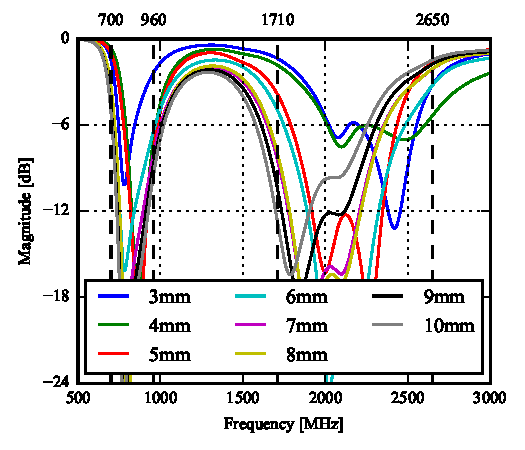
\includegraphics{img/tech_sol/monopole/5mm/s11_5mm}
        \caption{Efficiency for the top antenna, when sweeping the ground clearence.}
        \label{fig:eff_mono_sim_5mm}
    \end{subfigure}
    \caption{S11 and efficiency for the top antenna, when sweeping the ground clearence from \SI{3}{mm} to \SI{10}{mm}}
    \label{fig:eff_s11_mono_sim_5mm}
\end{figure}

Furthermore a sweep on the antenna hight was also carried out from \SI{7}{mm} to \SI{4}{mm}. The results are not included as the top antenna was unable to cover the high band at anything lower than \SI{7}{mm} in height.
